%#!platex -src-specials CategoryTheory.tex
\chapter{双対性}
これまでに,始対象と終対象,エピ射とモノ射というような,ある種の「双対性」
を示す定義の例を幾つかみてきた.今度は,そうした双対性をより体系的に考察
していこう.幾分自明な第一印象に反し,それこそが正に数学的構造に対する圏
論的なアプローチの深く強力な側面なのである.

\section{双対性原理}
手始めに,圏の形式的な定義をもう一度振り返っておこう.圏とは,対象$A, B,
C, \ldots$と射$f, g, h, \ldots$という二つの構成要素,そして四つの演算
$\dom(f), \cod(f), 1_A, g \circ f$があって,次の七つの公理を満たす物であっ
た.
\begin{equation}\label{CT}
 \begin{array}{rcl}
  \dom(1_A) = A              &   & \cod(1_A) = A\\
  f \circ 1_{\dom(f)} = f    &   & 1_{\cod(f)} \circ f = f\\
  \dom(g \circ f) = \dom(f)  &   & \cod(g \circ f) = \cod(g) \\
  h \circ (g \circ f)        & = & (h \circ g) \circ f
 \end{array}
\end{equation}
ここで,演算「$g \circ f$」は,
\[
 \dom(g) = \cod(f)
\]
のときのみ定義される.よって,$\circ$を含む等式には,
$\dom(g) = \cod(f) \Rightarrow \dom(g \circ f) = \dom(f)$
のように,この条件が適切な形で現れなくてはならない.

さて,$\Sigma$を圏の初等的な言語による文とすると,次の置換
\begin{align*}
 f \circ g & \text{ を} g \circ f\\
 \cod      & \text{ を} \dom\\
 \dom      & \text{ を} \cod
\end{align*}
によって「双対文」$\Sigma^{*}$を作ることが出来る.
この$\Sigma^{*}$も再びwell-formedな文となることは簡単に示せる.次に,
圏の公理を一切使わずに,$\Sigma$から$\Delta$を導くことが出来たとする.
即ち,$\Sigma \Rightarrow \Delta$としよう.すると,上の対応によって置換
された項は単なる未定義定数として扱うことが出来るので,明らかに
$\Sigma^{*} \Rightarrow \Delta^{*}$が成り立つ.ところで,圏論の
$(\ref{CT})$による公理系(CT)は,
\[
 \mathrm{CT}^* = \mathrm{CT}
\]
が成立するという意味において,それ自身「自己双対的」であることに注目しよ
う.すると,次の{\bfseries 双対性原理}を得る.

\begin{prop}[形式的な双対性]
 圏論の言語による任意の文$\Sigma$について,$\Sigma$が圏の公理のみから従
 うなら,その双対文$\Sigma^*$も同様に従う.つまり,
 \[
  \mathrm{CT} \Rightarrow \Sigma \;\text{ならば}
  \mathrm{CT} \Rightarrow \Sigma^*
 \]
 が成立する.
\end{prop}

より概念的な見方をしてみよう.文$\Sigma$がある対象と射の図式を含むとする.
\begin{center}
 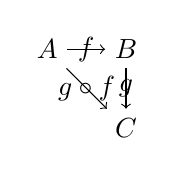
\begin{tikzpicture}
  \node (A) {$A$};
  \node (B) [right of=A]{$B$};
  \node (C) [below of=B]{$C$};

  \path[->]
    (A) edge node {$f$} (B)
        edge node [swap]{$g \circ f$} (C)
    (B) edge node {$g$} (C);
 \end{tikzpicture}
\end{center}
すると,双対文$\Sigma^*$は,その図式の射の向きと合成順を逆にしたものを含
むことに注目しよう.
\begin{center}
 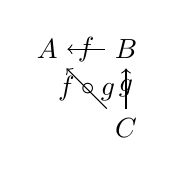
\begin{tikzpicture}
  \node (A) {$A$};
  \node (B) [right of=A]{$B$};
  \node (C) [below of=B]{$C$};

  \path[<-]
    (A) edge node {$f$} (B)
        edge node [swap]{$f \circ g$} (C)
    (B) edge node {$g$} (C);
 \end{tikzpicture}
\end{center}
圏${\bf C}$の逆圏${\bf C}^\mathrm{op}$を思い出せば,$\Sigma$ の${\bf C}$
での解釈は,自動的に$\Sigma^*$の${\bf C}^\mathrm{op}$での解釈を与えてい
ることがわかる.

さて,文$\Sigma$が任意の圏${\bf C}$で成立するとしよう.すると,$\Sigma$
は任意の圏${\bf C}^\mathrm{op}$でも成立し,従って$\Sigma^*$任意の圏
$({\bf C}^\mathrm{op})^{\mathrm{op}}$で成立する.しかし,任意の圏
${\bf C}$について,
\begin{equation}
  ({\bf C}^\mathrm{op})^{\mathrm{op}} = {\bf C}
\end{equation}
であるので,結局$\Sigma^*$も任意の圏${\bf C}$で成立することがわかる.従っ
て,次の概念的な形の双対性原理を得る.

\begin{prop}[概念的な双対性原理]
 圏論に関する文$\Sigma$が任意の圏で成立すれば,その双対文
 $\Sigma^*$も任意の圏で成立する.
\end{prop}

「終対象は同型を除いて一意である」といったような単純な,或いは自明な文し
かこの種の双対性の影響を受けないように見えるかもしれないが,実際にはそれ
以上の物である.これから見てゆくように,圏論的な双対性はとても強力で重要
な現象であることがわかる.射影幾何学での点と線の間の双対性のように,一つ
の証明から二つの定理を生む,「見返り」を効果的に倍増する物なのである.

そうした双対性は,任意の圏に関する主張を考える時だけではなく,むしろ「積
の図式である」といったような抽象的な構造や性質の定義に対して,その双対を
考えるときにも現れる.双対的な構造や性質は,合成順を入れ替えて「ドメイン」
「コドメイン」を取り替えることによって得られる.(或いは,元の性質を逆圏
で解釈することによっても同等の物が得られる.)\ref{余積}節では,そういっ
た種類の例を見る.
\section{余積}
\label{余積}
この章では,積の例とその双対概念が何であるかを考えてゆこう.初めに,積の
定義を思い出そう.
\begin{definition}
 図式$A \xleftarrow{p_1} P \xrightarrow{p_2} B$が$A$と$B$の{\bfseries 積}で
 あるとは,任意の$Z$と$A \xleftarrow{z_1} Z \xrightarrow{z_2} B$に対し,
 \begin{center}
  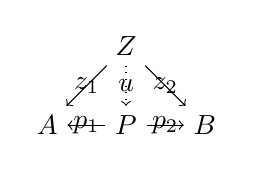
\begin{tikzpicture}
   \node (Z) {$Z$};
   \node (P) [below of=Z] {$P$};
   \node (A) [left  of=P] {$A$};
   \node (B) [right of=P] {$B$};
   \path[->]
     (Z) edge node [swap]{$z_1$} (A)
         edge node       {$z_2$} (B)
     (P) edge node       {$p_1$} (A)
         edge node [swap]{$p_2$} (B);
   \path[->, dotted] (Z) edge node {$u$} (P);
  \end{tikzpicture}
 \end{center}
 に示すような$p_i \circ u = z_i$を見たす$u: Z \to P$が一意に存在すること
 である.
\end{definition}

さて,この双対となる主張は何だろうか?

図式$A \xrightarrow{q_1} Q \xleftarrow{q_2} B$が$A$と$B$の「双対積」であ
るとは,任意の$Z$と$A \xrightarrow{z_1} Z \xleftarrow{z_2} B$に対し,
\begin{center}
  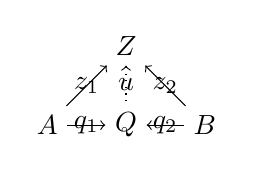
\begin{tikzpicture}
   \node (Z) {$Z$};
   \node (P) [below of=Z] {$Q$};
   \node (A) [left  of=P] {$A$};
   \node (B) [right of=P] {$B$};
   \path[<-]
     (Z) edge node [swap]{$z_1$} (A)
         edge node       {$z_2$} (B)
     (P) edge node       {$q_1$} (A)
         edge node [swap]{$q_2$} (B);
   \path[<-, dotted] (Z) edge node {$u$} (P);
  \end{tikzpicture}
\end{center}
に示すような$u \circ q_i = z_i$を見たす$u: Q \to Z$が一意に存在すること
である.実際,これらは{\bfseries 余積(coproduct)}と呼ばれる.このよう
に接頭辞「余(co-)」によって双対概念であることを示すという規約がある.通
常,余積は $A \xrightarrow{q_1} A+B \xleftarrow{q_2} B$と書き,一意射
$u: A+B \to Z$を $[f, g]$と書く.「余射影」$i_1: A \to A+B$と$i_2: B \to
A + B$は,通常{\bfseries 挿入射(入射;injection)}と呼ばれる.無論,挿入射は「単
射的(injective)」である必要はない.

従って,対象の余積は逆圏での積と一致する.もちろん,この対応によって余積
の例を多く得ることも出来る.しかし,他のもっと親しみのある例には何がある
のだろうか?

\begin{example}
 $\Sets$において,二つの集合の余積$A+B$はその非交和(disjoint union)であ
 り,例えば次のように構成できる.
 \[
  A + B = \Set{(a, 1) | a \in A} \cup \Set{(b, 2) | b \in B}
 \]
 ここで,挿入射は
 \[
  \begin{array}{ll}
   i_1(a) = (a, 1) & i_2(b) = (b, 2)\\
  \end{array}
 \]
 である.ここで,
\begin{center}
  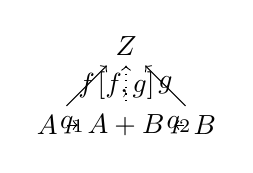
\begin{tikzpicture}
   \node (Z) {$Z$};
   \node (P) [below of=Z] {$A+B$};
   \node (A) [left  of=P] {$A$};
   \node (B) [right of=P] {$B$};
   \path[<-]
     (Z) edge node [swap]{$f$} (A)
         edge node       {$g$} (B)
     (P) edge node       {$q_1$} (A)
         edge node [swap]{$q_2$} (B);
   \path[<-, dotted] (Z) edge node {$\left[f,g\right]$} (P);
  \end{tikzpicture}
\end{center}
 のように任意の写像 $f, g$ が与えられたとき,$\left[f, g\right]$を次で定める.
 \[
  [f, g](x, \delta) =
 \begin{cases}
  f(x) & \delta = 1\\
  g(x) & \delta = 2
 \end{cases}
 \] % $
 このとき,$h \circ i_1 = f$ かつ $h \circ i_2 = g$となる$h$があれば,任
 意の$(x, \delta) \in A + B$について,
 \[
 h(x, \delta) = [f,g](x, \delta)
 \]
 とならなければならないことは簡単に計算できる.
\end{example}
$\Sets$において,任意の有限集合$A$は,
\[
A \cong 1 + 1 + \dots + 1 \;\;(n \text{回})
\]
のように余積で表せることに注意しよう(但し,$n = \mathrm{card}(A)$).こ
れは,写像$f: A \to Z$が各 $a \in A$に対する $f(a)$の値によって一意に
決定されることによる.従って,
\begin{align*}
 A &\cong \{a_1\} + \{a_2\} + \dots + \{a_n\}\\
   &\cong 1 + 1 + \dots + 1\;\;(n \text{回})
\end{align*}
が成立する.この類推で,単純に $2 = 1 + 1, 3 = 1 + 1 + 1$などとしばしば
略記する.

\begin{example}
 $M(A), M(B)$を集合$A, B$上の{\bfseries 自由}モノイドとするとき,$\Mon$
 でのこれらの余積を,
 \[
  M(A) + M(B) \cong M(A+B)
 \]
 として構成することが出来る.これは,$A+B$上の語を考えることで直接的に証
 明することもできるが,図式
 \begin{center}
  \begin{tikzpicture}
   \matrix (m) [matrix of math nodes, column sep=1.5cm, row sep=2cm] {
         & N      & \\
    M(A) & M(A+B) & M(B)\\
    A    &   A+B  & B\\
   };
   \path[->]
     (m-2-1) edge (m-1-2) edge (m-2-2)
     (m-2-3) edge (m-1-2) edge (m-2-2)
     (m-3-1) edge node {$\eta_A$} (m-2-1)
             edge (m-3-2)
     (m-3-2) edge node [swap] {$\eta_{A+B}$}(m-2-2)
     (m-3-3) edge node [swap]{$\eta_B$} (m-2-3)
             edge (m-3-2);
   \path[->, dotted] (m-2-2) edge (m-1-2);
  \end{tikzpicture}
 \end{center}
 を用いて抽象的に議論することも出来る.但し,各$\eta$は対応する生成元の
 埋め込みである.$M(A), M(B), A+B$および$M(A+B)$の普遍写像性によって,
 $M(A+B)$が$M(A) + M(B)$に必要な普遍写像性を持つことがわかる.ここで,
 $M(A)$と$M(B)$の余積$M(A) + M(B)$の元は,台集合の元の余積{\bfseries で
 はなく},単にそれらの生成元の余積 $A+B$から{\bfseries 生成されている}こ
 とに注意しよう.必ずしも自由とは限らない任意のモノイドにの余積について
 は,すぐ後で考察する.

 上の例は,自由モノイド函手$M: \Sets \to \Mon$が余積を保存することを示し
 ている.これは,後程考察するより一般的な現象の一例であり,既に見た忘却
 函手$U: \Mon \to \Sets$が表現可能函手であり従って積を保存する事実と関連
 している.
\end{example}

\begin{example}\label{ex:Coproduct in Top or Pos}
 ${\bf Top}$において,二つの空間の余積
 \[
  X + Y
 \]
 は,それらの非交和に$O(X+Y) \cong O(X) \times O(Y)$によって位相を入れた
 ものになる.これは,離散空間の$O(X) = \Pow(X) \cong 2^X$のパターンに従っ
 たものであることに注意しよう.つまり,離散空間については実際に,
 \[
  O(X+Y) \cong 2^{X+Y} \cong 2^X \times 2^Y \cong O(X) \times O(Y)
 \]
 が成立する.

 これと関連する事実は,二つの冪集合ブール代数$\Pow(A)$と$\Pow(B)$の積が
 再び冪集合となること,即ち$A$と$B$の余積の冪集合となることである:
 \[
  \Pow(A) \times \Pow(B) = \Pow(A + B)
 \]
 このことを確かめるのは演習問題とする.

 posetの余積も,台集合の余積と同じように「隣同士に並べておく」ことによっ
 て得られる.では,区別された始元$0$を持つ「根付き(rooted)」posetの場合
 はどうだろうか?そのようなposetと$0$を保存する単調写像の圏$\Pos_0$では,
 そのようなposet $A, B$ の余積を,poset の圏$\Pos$での余積$A+B$で異なる
 $0$を「同一視」した
 \[
  A +_{\Pos_0} B \cong (A +_{\Pos} B)/ ``0_A = 0_B ''
 \]
 として構成できる.すぐ後で,こうした同一視(同値関係の商)を「コイコラ
 イザ」として説明する方法を見る.
\end{example}

\begin{example}
 $P$ を poset とし,任意に一つ固定する.二元$p, q \in P$の$P$での余積は
 何だろうか?
 \[
  \begin{array}{ll}
   p \leq p + q& q \leq p + q
  \end{array}
 \]
 が成り立たねばならず,更に
 \[
  p \leq z \;\; \text{かつ} \;\; q \leq z
 \]
 ならば,
 \[
  p+q \leq z
 \]
 でなければならない.よって,$p + q = p \vee q$ は$p$と$q$の「結び(join)」
 あるいは「最小上界」である.
\end{example}

\begin{example}
 $\ref{Sec:Example of Categories}$節の例$\ref{example of logic}$で出て
 来た論理学における演繹系の{\bfseries 証明の圏}では,通常の自然演繹の選
 言の導入・除去規則から余積が出て来る.特に,導入規則
\[
 \begin{array}{ll}
  \AxiomC{$\varphi$}
  \UnaryInfC{$\varphi \vee \psi$}
  \DisplayProof{}
  &
  \AxiomC{$\psi$}
  \UnaryInfC{$\varphi \vee \psi$}
  \DisplayProof{}
 \end{array}
\]
 が射
 $i_1: \varphi \to \varphi \lor \psi$ と $ i_2: \psi \to \varphi \lor \psi$
 を定め,除去規則
 \begin{prooftree}
  \AxiomC{$\varphi \lor \psi$}
  \AxiomC{$[\varphi]$}
  \noLine
  \UnaryInfC{$\vdots$}
  \noLine
  \UnaryInfC{$\vartheta$}
  \AxiomC{$[\psi]$}
  \noLine
  \UnaryInfC{$\vdots$}
  \noLine
  \UnaryInfC{$\vartheta$}
  \TrinaryInfC{$\vartheta$}
 \end{prooftree}
 が二つの射$p:\varphi \to \vartheta, q: \psi \to \vartheta$に対する
 $[p, q]: \varphi \lor \psi \to \vartheta$を与える.しかし,射の同値性を
 証明の同値性として定義しているため,必要な等式
\begin{equation}
   \begin{array}{ll}
   [p, q] \circ i_1 = p& [p, q] \circ i_2 = q
  \end{array}\label{余積条件}
\end{equation} 
 は明らかに成立しない.余積を得るためには,上のような等式と,任意の
 $r: \varphi \lor \psi \to \vartheta$に対する補足的な等式
 \begin{equation}
  [r \circ i_1, r \circ i_2] = r
 \end{equation}
 から生成される同値関係による同値類を経由することで,等式が成立するよう
 に「強制」しなくてはならない(直観的には,そのような「脇道」を省略した
 ときに同じと見做せるような証明を全て同一視してやる,ということである).
 証明の同値類を射とした新たな圏では,射$[p, q]$も$(\ref{余積条件})$を満た
 すような{\bfseries 一意的な}射となるので,実際に$\varphi \lor \psi$は余
 積となる.

 (注意$\ref{Curry-Howard}$のCurry-Howard対応を通して)この例と密接に関
 連しているのは,通常\verb|case|項を用いて定式化される,$\lambda$計算の
 直和型である.これらは$\ref{直積の例}$節で定義した{\bfseries 型の圏}で
 の余積となっている.
\end{example}

\begin{example}
 任意の二つのモノイド$A, B$は,
 \[
  A + B = M(|A| + |B|)/\sim
 \]
 の形の余積を持つ.これまでと同様,自由モノイド$M(|A| + |B|)$は$A, B$の
 台集合の非交和上の文字列(語),すなわち$A$と$B$の両方の元からなる文字
 列であり,また同値関係$v \sim w$は,次の等式群を含む最小の同値関係であ
 る.
 \begin{align*}
  (\ldots x u_A y \ldots) &= (\ldots x y \ldots)\\
  (\ldots x u_B y \ldots) &= (\ldots x y \ldots)\\
  (\ldots a a' \ldots)    &= (\ldots a \cdot a' \ldots)\\
  (\ldots b b' \ldots)    &= (\ldots b \cdot b' \ldots)
 \end{align*}
 (もし同値関係で集合を割るということの復習が必要であれば,以後の記述を
 飛ばして$\ref{コイコライザ}$節の冒頭を先に読んで頂きたい.)単位元は,
 もちろん空語の同値類$[-]$である(これは$[u_A]$および$[u_B]$に等しい).
 同値類の積は,期待される通りの方法,即ち
 \[
  [x \ldots y] \cdot [x' \ldots y']
   = [x \ldots y x' \ldots y']
 \]
 によって定められる.余積の挿入射$i_A: A \to A+B$と$i_B:B \to A+B$は,単
 に
 \[
  \begin{array}{ll}
   i_A(a) = [a],&  i_B(b) = [b]
  \end{array}
 \]
 であり,これらが準同型となることは容易に確かめられる.モノイド$M$への準
 同型$f: A \to M$と$g: B \to M$が与えられたとき,一意的な射
 \[
  [f, g]: A + B \to M
 \]
 は次のようにして得られる.まず,写像
 \[
  [|f|, |g|]: |A| + |B| \to |M|
 \]
 を,自由モノイド$M(|A| + |B|)$上の準同型$[f, g]'$に拡張する.
 \begin{center}
  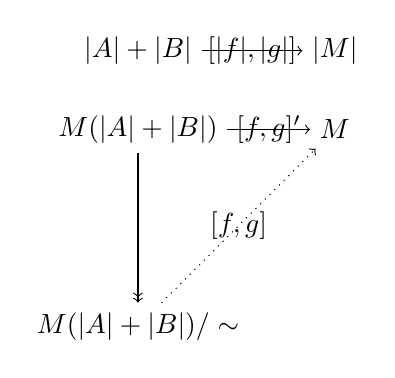
\begin{tikzpicture}[]
    \node (absAB)   at (0cm,3.5cm) {$|A| + |B|$};
    \node (absM)    at (2.5cm,3.5cm) {$|M|$};
    \node (MabsAB)  at (0cm,2.5cm) {$M(|A|+|B|)$};
    \node (M)       at (2.5cm,2.5cm) {$M$};
    \node (MABquot) at (0cm,0cm) {$M(|A|+|B|)/\sim$};
   
   \path[->] (absAB) edge node {$[|f|,|g|]$} (absM);
   \path[->] (MabsAB) edge node {$[f,g]'$} (M);
   \path[->>] (MabsAB) edge (MABquot);
   \path[->, dotted] (MABquot) edge node[swap] {$[f,g]$} (M);
  \end{tikzpicture}
 \end{center}
 すると,$[f, g]'$は「同値関係$\sim$を保つ」こと,即ち$M(|A|+|B|)$で
 $v\sim w$が成り立てば$[f, g]'(v) = [f, g]'(w)$となることがわかる.した
 がって,写像$[f, g]'$は商集合へと拡張でき,求める写像
 $[f, g]:M(|A|+|B|)/\sim \to M$を得る.(この写像が$hi_A = f$かつ
 $hi_B=g$を満たす一意な準同型となるのは何故か?)従ってまとめれば,
 \[
  A + B \cong M(|A|+|B|)/\sim
 \]
 を得る.

 この構成は,${\bf Groups}$での余積を与えるのにも用いることが出来る.
 通常,${\bf Groups}$での余積は,他の「代数」,つまり演算の入った集合と
 同様に$A$と$B$の{\bfseries 自由積}と呼ばれ,$A \oplus B$などと書く.再
 び,自由モノイドのときと同様に,$A+B$の台集合は集合としての$A, B$の余積
 とは一致しない(忘却函手$\Mon \to \Sets$は余積を保存しない).
\end{example}

\begin{example}
 アーベル群$A, B$について,自由積$A \oplus B$はアーベル群であるとは限ら
 ない.勿論,更に$A \oplus B$の商を取ることでアーベル群の圏${\bf A}$の余
 積になるようにすることは出来るが,より便利な(かつ重要な)表示法がある
 ので,以下ではそれを見てゆこう.

 自由積$A\oplus B$の語は,更に可換性の条件
 \[
  (a_1 b_1 a_2 b_2) \sim (a_1 a_2 \ldots b_1 b_2 \ldots)
 \]
 を満たさなればならないので,語を入れ換えて,全ての$a$を語の先頭,$b$を
 末尾に持ってくることが出来る.ところが,更に
 \[
  (a_1 a_2 \ldots b_1 b_2 \ldots)
    = (a_1 + a_2 + \ldots + b_1 + b_2 + \ldots)
 \]
 が既に成立しているので,実際には元の対$(a, b)$が与えられているのと等価
 である.従って,余積の台集合として,{\bfseries 積}
 \[
  |A+B| = |A\times B|
 \]
 を取ることが出来る.挿入射には準同型
 \begin{align*}
  i_A(a) &= (a, 0_B)\\
  i_B(b) &= (0_A, b)
 \end{align*}
 を用いる.このとき,任意の準同型 $A \xrightarrow{f} X \xleftarrow{g} B$
 が与えられたとき,$[f, g]: A+B \to X$ を次で定義することが出来る.
 \[
  [f, g](a, b) = f(a) +_X g(b)
 \]
 この定義で実際うまくゆくことは簡単にわかるだろう(演習問題!).

 更に,台{\bfseries 集合}が一致するだけではなく,アーベル群の積と余積は,
 実際に{\bfseries 群}として同型になるのである.
 \begin{prop}
  アーベル群の圏${\bf Ab}$において,二項余積と積の間には自然な同型
  \[
   A + B \cong A \times B
  \]
  が存在する.
 \end{prop}
 \begin{proof}
  射 $\vartheta: A + B \to A \times B$を定義する為には,射
  $A \to A \times B$(と$B \to A \times B$)が必要であり,従って射
  $A \to A$ と $A \to B$(そして$B \to A$と$B \to B$)が必要となる.そこ
  で,それぞれに対応するものとして $1_A : A \to A$と零準同型$0_B:A\to B$
  (および$0_A: B \to A$と$1_B: B \to B$)を取る.これらを全て合わせて,
  \[
   \vartheta = [\langle 1_A, 0_B\rangle, \langle 0_A, 1_B\rangle]
             : A + B \to A \times B
  \]
  を得る.ここで任意の$(a,b) \in A+B$を取れば,
  \begin{align*}
   \vartheta(a,b)
   &= [\langle 1_A, 0_B\rangle, \langle 0_A, 1_B\rangle](a,b)\\
   &= \langle 1_A, 0_B\rangle(a) + \langle 0_A, 1_B\rangle](b)\\
   &= (1_A(a), 0_B(a)) + (0_A(b), 1_B(a))\\
   &= (a, 0_B) + (0_A, b)\\
   &= (a + 0_A, 0_B + b)\\
   &= (a, b)
  \end{align*}
  となる.
 \end{proof}
 この事実はMacLaneによって最初に確認され,二つのアーベル群(そして加群や
 ベクトル空間など関連する構造)の間の平行な射$f, g: A \to B$の二項加法演
 算へと繋がる概念であることが示された.事実,特定のアーベル群$A$の群構造
 は,$A$への射に対する演算から復元することが出来るのである.より一般に,
 そうした射の間の加法演算の存在は, ${\bf Ab}$のような「アーベル圏」と呼
 ばれる圏の抽象的説明の土台として用いることが出来る.アーベル圏は公理的
 ホモロジー論と相性がよい.

 積の場合とちょうど同様に,空の余積を考えることが出来,それは始対象$0$である.
 また,複数因子の余積も定義出来るし,二つの射の余積
 \[
  f+f': A + A' \to B + B'
 \]
 も定義できて,そこから二項余積を持つ圏${\bf C}$上の余積函手
 $+: {\bf C} \times {\bf C} \to {\bf C}$が導出される.
 こうした事実は,すべて双対性から簡単に出て来るものである.つまり,双対
 概念を逆圏で考えることによって出てくる.同様にして,次の命題が得られる.
 \begin{prop}
  余積は同型を除き一意である.
 \end{prop}
 \begin{proof}
  双対性と「同型射」の双対は「同型射」であるという事実を使えばよい.
 \end{proof}
 ちょうど同じようにして,二項直積は同型を同一視すれば結合的であることも示す
 ことが出来る.

 よって,今後は,ある双対概念が元の概念と似た(しかし双対的な)性質を持
 つこと示すのに,一度新たな概念を導入してそれを単純に観察することに帰着
 されることが一般的となる.\ref{Sec:Equalizer}および
 \ref{Sec:Coequalizer}節では,更にもうひとつこの種の例を見ていく.
\end{example}
\section{イコライザ}

この節では,また別の抽象的特徴付けについて考察する.今回見てゆくのは,実
数値函数の零点集合といったような等式によって定義された「代数多様体」や,
準同型写像の核などに共通な性質の一般化である.これは,集合論の分出公理に
似たようなものでもある.

\begin{definition}
 任意の圏${\bf C}$において,二つの平行な射
 \begin{center}
  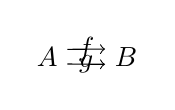
\begin{tikzpicture}
   \node (A) {$A$};
   \node (B) [right of=A] {$B$};
   \path[->] (A.20) edge node {$f$} (B.160)
             (A.340) edge node [swap]{$g$} (B.200);
  \end{tikzpicture}
 \end{center}
 が与えられているとする.このとき,$f$ と $g$の{\bfseries イコライ
 ザ}({\itshape equalizer})とは,対象$E$と射$e:E \to A$ から成り,以下が
 普遍的に成り立つことである:
 \[
  f \circ e = g \circ e
 \]
 つまり,$f \circ z = g \circ z$を見たすような$z: Z \to A$が与えられたと
 き,$e \circ u = z$となるような射$u: Z \to E$が一意的に存在するというこ
 とである.それはちょうど次の図のように表すことが出来る.
 \begin{center}
  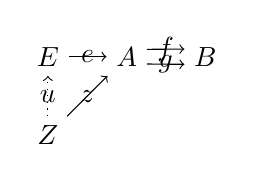
\begin{tikzpicture}
   \node (E) {$E$};
   \node (A) [right of=E] {$A$};
   \node (B) [right of=A] {$B$};
   \node (Z) [below of=E] {$Z$};

   \path[->]
     (E) edge node {$e$} (A)
     (A.20)  edge node {$f$} (B.160)
     (A.340) edge node [swap]{$g$} (B.200)
     (Z) edge node [swap] {$z$} (A);
   \path[->, dotted] (Z) edge node {$u$} (E);
  \end{tikzpicture}
 \end{center}
\end{definition}
では,幾つか単純な例を見てみよう.

\begin{example}
 次のような函数$f, g: \R^2 \rightrightarrows \R$があったとする.
 \begin{align*}
  f(x,y) &= x^2 + y^2\\
  g(x,y) &= 1
 \end{align*}
 今,これらのイコライザを,例えば${\bf Top}$で取るとしよう.それは部分空間
 \[
  S = \Set{(x, y) \in \R^2 | x^2 + y^2 = 1} \hookrightarrow \R^2
 \]
 であり,つまりは$xy$平面上の単位円である.任意の「一般化元」
 $z: Z \to \R^2$ について,二つの射影とそれぞれ合成してやることで
 $z = \langle z_1, z_2 \rangle$ なる二つの「元」$z_1, z_2: Z \to R$ を得
 ることが出来る.また,これらについて
 \begin{align*}
  f(z) = g(z) &\iff z_1^2 + z_2^2 = 1\\
              &\iff ``\langle z_1, z_2 \rangle = z \in S ''
 \end{align*}
 が成立する.ここで,最終行は実際には包含写像$i: S \hookrightarrow \R^2$
 を介した因数分解$z = \bar{z} \circ i$ が存在しているということを意味い
 している.次の図式がこの状況をよく表している.
 \begin{center}
  \begin{tikzpicture}
   \node (S) {$S$};
   \node (R^2) [right of=S] {$\R^2$};
   \node (R) [right of=R^2] {$\R$};
   \node (Z) [below of=S] {$Z$};
   \path[right hook->] (S) edge node {$i$} (R^2);
   \path[->, dotted] (Z) edge node {$\bar{z}$} (S);
   \path[->]
     (Z) edge node [swap] {$z$} (R^2)
     (R^2.15)  edge node {$x^2+y^2$} (R.160)
     (R^2.345) edge node [swap]{$1$} (R.200);
  \end{tikzpicture}
 \end{center}
 包含写像$i$はモニックなので,このような因数分解がもし存在すれば一意であ
 り,従って$S \hookrightarrow \R^2$は実際に$f$ と $g$のイコライザとなる.
\end{example}

\begin{example}
 同様に,$\Sets$における任意の写像$f, g: A \rightrightarrows B$のイコラ
 イザは,等式的に定義される部分集合
 \[
  \Set{ x \in A | f(x) = g(x)} \hookrightarrow A
 \]
 から $A$ への包含写像である.この議論は先程のものと本質的に同じものであ
 る.

 ここで,どんな部分集合$U \subseteq A$もこのような「等式的な」形で書き下
 せること,つまり,任意の部分集合はある二つの写像のイコライザと
 して表せるということに注意したい.実際,これはごく自然な方法によって確
 かめることが出来る.まず,
 \[
  2 = \Set{\top, \bot}
 \]
 とし,これを「真理値」の集合と考える.つづいて,$x \in A$に対し,
 \[
  \chi_U(x) = \begin{cases}
	       \top & x \in U\\
	       \bot & x \notin U
	      \end{cases}
 \]
 で定められる{\bfseries 特性函数}({\itshape characteristic function})
 \[
  \chi_U : A \to 2
 \]
 を考える.このとき,
 \[
  U = \Set{x \in A | \chi_U(x) = \top}
 \]
 が成立する.よって,次の図式がイコライザとなる.
 \begin{center}
  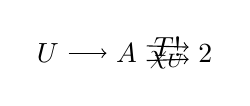
\begin{tikzpicture}
   \node (U) {$U$};
   \node (A) [right of=U] {$A$};
   \node (2) [right of=A] {$2$};
   \path [->]
     (U) edge (A)
     (A.20)  edge node {$T!$} (2.160)
     (A.340) edge node [swap] {$\chi_U$} (2.200);
  \end{tikzpicture}
 \end{center}
 ここで,$T! = T \circ ! : U \xrightarrow{!} 1 \xrightarrow{T} 2$ である.

 更に,任意の写像
 \[
  \varphi : A \to 2
 \]
 に対し,「代数多様体」(すなわち等式による部分集合)
 \[
  V_\varphi = \Set{ x \in A | \varphi(x) = \top}
 \]
 を考えることができ,これもまたイコライザとなる.($\varphi$を$A$上の「命
 題函数」と考えることで,部分集合$V_\varphi \subseteq A$は分出公理が保証
 する$\varphi$の「外延」と見做すことが出来る.)

 さて,これらの操作$\chi_U, V_\varphi$が互いに逆演算となっていることは次
 のように容易にわかる.
 \begin{align*}
  V_{\chi_U} &= \Set{x \in A | \chi_U(x) = \top}\\
             &= \Set{x \in A | x \in U}\\
             &= U
 \end{align*}
 また,任意の$U \subseteq A$について,任意の$\varphi: A \to 2$が
 与えられれば,
 \begin{align*}
  \chi_{V_\varphi}(x) &= \begin{cases}
			  \top & x \in V_\varphi\\
			  \bot & x \notin V_\varphi
			 \end{cases}\\
  &= \begin{cases}
      \top & \varphi(x) = \top\\
      \bot & \varphi(x) = \bot
     \end{cases}\\
  &= \varphi(x)
 \end{align*}
 以上のようにイコライザを取ることを通して,お馴染の同型
 \[
  \Hom(A, 2) \cong \Pow(A)
 \]
 を得ることができる.
\end{example}

写像のイコライザとして部分集合を取ることが出来るという事実は,更に一般
的な現象の特別な場合にすぎない.

\begin{prop}\label{Prop:Equalizer is Monic}
 任意の圏において,もし$e: E \to A$が何らかの射の組のイコライザであれば,
 $e$ はモノ射である.
\end{prop}
\begin{proof}
 以下の図式を考える.
 \begin{center}
  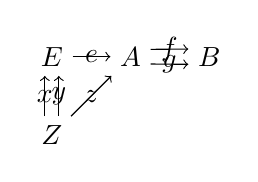
\begin{tikzpicture}
   \node (E) {$E$};
   \node (A) [right of=E]{$A$};
   \node (B) [right of=A]{$B$};
   \node (Z) [below of=E]{$Z$};

   \path[->]
     (E)     edge node {$e$} (A)
     (A.20)  edge node {$f$} (B.160)
     (A.340) edge node [swap] {$g$} (B.200)
     (Z) edge node [swap]{$z$} (A)
     (Z.70) edge node [swap]{$y$} (E.290)
     (Z.110) edge node {$x$} (E.250);
  \end{tikzpicture}
 \end{center}
 ここで,$e$は$f$と$g$のイコライザであるとする.$ex = ey$を仮定して,
 $x = y$を示す.$z = ex = ey$とおく.すると,$fz = fex = gey = gz$となり,
 従って$eu = z$なる$u: Z \to E$が{\bfseries 一意的に}存在する.よって,
 $ex = z$および$ey = z$から $x = u = y$が従う.
\end{proof}

\begin{example}
 poset の圏やモノイドの圏など他の多くの圏において,二つの射
 $f, g: A \rightrightarrows B$のイコライザは上のように台写像のイコライザ
 を取ることで構成できる.つまり,$f$と$g$が一致する元($f(x) = g(x)$とな
 る元)$x \in A$からなる部分集合$A(f=g) \supseteq A$を取り,$A$の構造を
 $A(f=g)$に制限してやればよいのである.例えば,posetに対しては$A$の順序
 を$A(f=g)$に制限したものを,位相空間に対しては部分空間位相をそれぞれ取っ
 てやればよい.

 モノイドの圏では,部分集合$A(f=g)$は$A$の演算により再びモノイドとなるの
 で,包含写像は準同型写像となる.何故ならば,$f(u_A) = u_B = g(u_A)$であるこ
 と,また $f(a) = g(a)$かつ$f(a') = g(a')$ならば
 $f(a \cdot a') = f(a) \cdot f(a') = g(a) \cdot g(a') = g(a \cdot a')$
 となることから,$A(f=g)$は単位元を持ち積について閉じることがわかるから
 である.

 例えば,特にアーベル群であれば,
 \[
  f(x) = g(x) \iff (f - g)(x) = 0
 \]
 という事実を用いて上とは異なった説明を考えることが出来る.
 $f$と$g$のイコライザは準同型$(f-g)$と零準同型$0: A \to B$のイコライザと
 同じものになるので,従って任意の準同型$h: A\to B$に対して
 $A(h, 0) \mono A$の形のイコライザを考えれば充分である.この$A$の部分群
 を$h$の{\bfseries 核}({\itshape kernel})と呼び,$\mathrm{ker}(h)$と書
 く.以上から,イコライザ
 \begin{center}
  \begin{tikzpicture}
   \node (ker) {$\mathrm{ker}(f - g)$};
   \node (A) [right of=ker] {$A$};
   \node (B) [right of=A]   {$B$};
   \path[right hook->] (ker) edge (A);
   \path[->]
     (A.20)  edge node {$f$} (B.160)
     (A.340) edge node [swap] {$g$} (B.200);
  \end{tikzpicture}
 \end{center}
 を得る.準同型の核は群の研究の根幹を成す重要な概念であり,第
 \ref{Ch:Groups and Categories}章で詳しく考察する.
\end{example}
\label{Sec:Equalizer}
\section{コイコライザ}
\label{Sec:Coequalizer}
コイコライザは同値関係による商の概念の一般化である.そこで,既に何度か使っ
てきたこの概念を復習することから始めよう.まず,集合$X$上の{\bfseries 同
値関係}({\itshape equivalence relation})とは,次の三条件を満たす二項関係
$x \sim y$のことであったことを思い出そう.
\begin{quote}
 反射律:$x \sim x$\\
 対称律:$x \sim y \implies y \sim x$\\
 推移律:$x \sim y \text{かつ} y \sim z \implies x \sim z$
\end{quote}
同値関係が与えられたとき,元$x \in X$の{\bfseries 同値類}
({\itshape equivalence class})$[x]$を
\[
 [x] = \Set{y \in X | x \sim y}
\]
によって定める.すると,種々の異なる同値類$[x]$は$X$の{\bfseries 分
割}({\itshape partition})を与える.つまり,各元$y$はそのような同値類のう
ちただ一つだけに属し,即ちそれが$[y]$である(示せ!).

同値関係は,ある性質を共通に持つ元(例えば同じ色であるとか)から得られる
と考えることがある.すると,同値類$[x]$はそうした性質として見做すことが
出来,その意味で「抽象的な対象」(赤や青などの色それ自身など)と見ること
が出来る.こうした手法は「抽象化による定義」として知られている.例えば,
実数を有理数のCauchy列から構成する方法や,有限集合から有限基数を構成する
方法の説明として用いられる.

全ての同値類の集合
\[
 X/\sim = \Set{[x] | x \in X}
\]
は$X$の$\sim$による{\bfseries 商}({\itshape quotient})としばしば呼ばれ
る.商集合は,同値な元$x \sim y$の違いを「捨象」したいときに$X$の代わり
に使われる.何故なら,
\[
 [x] = [y] \iff x \sim y
\]
が成立するので,$X/\sim$では$x \sim y$を満たす元(だけ)が同一視されるか
らである.ここで,$x$を$[x]$に移す{\bfseries 商写像}({\itshape quotient
mapping})
\[
 q: X \to X / \sim
\]
の持つ性質に注目してみよう.写像$f: X \to Y$は,$f$が同値関係を保つとき
に限り,つまり$x \sim y$ならば$f(x) = f(y)$が成り立つときに限り,下図の
ように$q$に沿って拡張することが出来るのである.
\begin{center}
 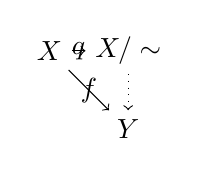
\begin{tikzpicture}
  \node (X) {$X$};
  \node (Xq) [right of=X] {$X/\sim$};
  \node (Y) [below of=Xq] {$Y$};
  \path[->]
    (X) edge node {$q$} (Xq)
        edge node [swap]{$f$} (Y);
  \path[->, dotted] (Xq) edge (Y);
 \end{tikzpicture}
\end{center}

それでは,イコライザの双対概念であるコイコライザについて考えよう.

\begin{definition}
 圏${\bf C}$の平行な射$f, g: A \to B$の{\bfseries コイコライ
 ザ}({\itshape coequalizer})とは,$Q$と次の図式に示すような
 $qf = qg$を満たすような普遍射$q: B \to Q$の組のことである.

 \begin{center}
  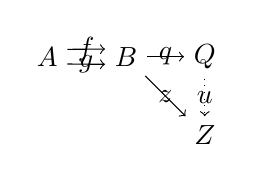
\begin{tikzpicture}
   \node (A) {$A$};
   \node (B) [right of=A] {$B$};
   \node (Q) [right of=B] {$Q$};
   \node (Z) [below of=Q] {$Z$};
   \path[->]
     (A.20)  edge node        {$f$} (B.160)
     (A.340) edge node [swap] {$g$} (B.200)
     (B)     edge node        {$q$} (Q)
             edge node [swap] {$z$} (Z);
   \path[->, dotted] (Q) edge node {$u$} (Z);
  \end{tikzpicture}
 \end{center}
 つまり,任意の$Z$と$zf = zg$を見たす$z: B \to Z$が与えられたとき,
 $uq = z$なる射$u: Q \to Z$が一意に存在することである.
\end{definition}

まず,双対性から${\bf C}$のイコライザ$q$は${\bf C}^\op$でイコライザとな
り,命題$\ref{Prop:Equalizer is Monic}$からモニックとなるので,従って$q$
は ${\bf C}$でエピックとなることがわかる.

\begin{prop}
 もし$q: B \to Q$がある射の組のコイコライザであれば,$q$はエピ射である.
\end{prop}

従って,コイコライザ$q: B \epi Q$は,$f(a) = g(a)$によって
(もし「元」$a \in A$があれば)同じ元からの行き先を全て「同一視」して,
$B$を「つぶした」ものと考えることができる.単につぶすだけではなく,そう
した同一視を保ちつつ任意の$Z$へと移せるように,$B$を限りなく小さ
く「極小」になるようにつぶしたものである.

\begin{example}
 $R \subseteq X \times X$を集合$X$上の同値関係として,図式
 \begin{center}
  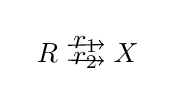
\begin{tikzpicture}
   \node (R) {$R$};
   \node (X) [right of=R]{$X$};
   \path[->]
     (R.20)  edge node        {$r_1$} (X.160)
     (R.340) edge node [swap] {$r_2$} (X.200);
  \end{tikzpicture}
 \end{center}
 を考えよう.ここで,$r_1, r_2$は$R \subseteq X \times X$の包含写像の二
 つの射影
 \begin{center}
  \begin{tikzpicture}
   \node (R)                  {$R$};
   \node (XxX) [below of=R]   {$X \times X$};
   \node (X1)  [left of=XxX]  {$X$};
   \node (X2)  [right of=XxX] {$X$};
   \path[->]
    (R)   edge node [swap] {$r_1$} (X1)
          edge node        {$r_2$} (X2)
    (XxX) edge node        {$p_1$} (X1)
          edge node [swap] {$p_2$} (X2);
   \path[left hook->] (R) edge (XxX);
  \end{tikzpicture}
 \end{center}
 である.

 このとき,$x \mapsto [x]$で定める商射影
 \[
  \pi: X \to X/R
 \]
 は$r_1$と$r_2$のコイコライザとなる.次の図式に示すような$f: X \to Y$が
 与えられたとする.
 \begin{center}
  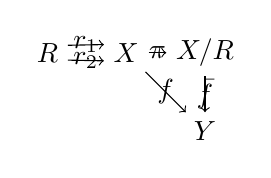
\begin{tikzpicture}
   \node (R)                {$R$};
   \node (X)  [right of=R]  {$X$};
   \node (XR) [right of=X]  {$X/R$};
   \node (Y)  [below of=XR] {$Y$};
   \path[->]
     (R.20)  edge node        {$r_1$}     (X.160)
     (R.340) edge node [swap] {$r_2$}     (X.200)
     (XR)    edge node        {$\bar{f}$} (Y)
     (X)     edge node        {$\pi$}     (XR)
             edge node [swap] {$f$}       (Y);
  \end{tikzpicture}
 \end{center}
 すると,既にみたように,$f$が$R$を保存すれば,即ち$(x, x') \in R$ならば
 $f(x) = f(x')$が成立するならば,
 \[
  \bar{f}\pi(x) = f(x)
 \]
 を見たすような写像$\bar{f}$が存在する.ところが,
 $f \circ r_1(x, x') = f(x)$かつ$f \circ r_2(x,x') = f(x')$が
 $(x, x') \in R$について成立するので,この条件は結局
 $f\circ r_1 = f \circ r_2$ということを述べていることになる.更に,$\pi$
 はエピ射なので,もしそのような$\bar{f}$が存在すれば必然的に一意である.

 $\Sets$における任意の二本の平行射$f, g: A \rightrightarrows B$ のコイコ
 ライザは,各$x \in A$に対して$f(x) = g(x)$の形の等式から生成される同値
 関係で$B$を割ったものとして得られる.この詳細は演習問題としよう.
\end{example}

\begin{example}
 例$\ref{ex:Coproduct in Top or Pos}$では,{\bfseries 根つき}poset $P$と
 $Q$の余積を,まずposetの圏で$P+Q$をとり,二つの異なる零元
 $0_P$ と $0_Q$を(つまり挿入射によるそれぞれの像を)「同一視」すること
 で構成した.今や,この「同一視」はposetの圏でのコイコライザ
 \begin{center}
  \begin{tikzpicture}
   \matrix (m) [matrix of math nodes, column sep=1cm, row sep=1cm] {
     1 & P+Q & X+Q/(0_P = 0_Q) \\
   };
   \path[->]
     (m-1-1.20)  edge node        {$0_P$} (m-1-2.170)
     (m-1-1.340) edge node [swap] {$0_Q$} (m-1-2.185)
     (m-1-2)     edge                     (m-1-3);
  \end{tikzpicture}
 \end{center}
 として説明することが出来る.これは明らかに{\bfseries 根つき}posetの余積
 の普遍写像性を持つ.

 位相幾何学でも,(例えば区間の端点を同一視して円をつくるように)点を
 「同一視」したり,(平面上の領域からトーラスを構成するように)部分空間
 を「同一視」したりする.こうした例や,多くの似たような「貼り付け」によ
 る構成はコイコライザとして説明することが出来る.
 ${\bf Top}$では,写像の平行対$f, g: X \to Y$のコイコライザは$Y$の商空間
 として構成できる(演習を参照).
\end{example}

\begin{example}[代数の表示]\label{FinPresAlg}
 群やモノイドのような「代数系」,つまり(有限引数の)演算が入った集合か
 らなる任意の圏を考えよう.後で,そうした圏は任意の集合に対する自由代数
 を持ち,任意の射の平行対に対するコイコライザを持つことを示す(モノイド
 の圏がコイコライザを持つことは演習問題を見よ).こうした事実を用いて,
 代数系の{\bfseries 生成元}({\itshape generator})と{\bfseries 関係式}
 ({\itshape relations})による{\bfseries 表示}({\itshape presentation})を
 決定することができる.例えば,次が与えられたとしよう:
 \begin{equation}
   \begin{array}{l}
  \text{生成元}: x, y, z\\
  \text{関係式}: xy = z, y^2 = 1\label{生成元と関係式}
   \end{array}
 \end{equation}
 こうした生成元と関係式による代数系を構築するために,自由代数
 \[
  F(3) = F(x, y, z)
 \]
 から始めて,次に写像のコイコライザ
 \begin{center}
  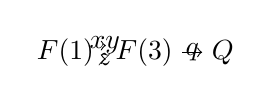
\begin{tikzpicture}
   \node (F1)               {$F(1)$};
   \node (F3) [right of=F1] {$F(3)$};
   \node (Q)  [right of=F3] {$Q$};

   \path[->]
     (F1.10)  edge node        {$xy$} (F3.170)
     (F1.350) edge node [swap] {$z$}  (F3.190)
     (F3)     edge node        {$q$}  (Q);
  \end{tikzpicture}
 \end{center}
 を取ることで,関係式$xy = z$が成立するように「強制」しよう.ここで,
 $F(1)$の生成元を$v$としたとき,$v \mapsto a$によって写像$F(1) \to A$が
 元$a \in A$に対応するという事実を使った.また,同様にして等式$y^2 = 1$
 に対しても,コイコライザ
 \begin{center}
  \begin{tikzpicture}
   \node (F1)               {$F(1)$};
   \node (Q)  [right of=F1] {$Q$};
   \node (Q') [right of=F3] {$Q'$};

   \path[->]
     (F1.10)  edge node        {$q(y^2)$} (Q.160)
     (F1.350) edge node [swap] {$q(1)$}   (Q.195)
     (F3)     edge                        (Q');
  \end{tikzpicture}
 \end{center}
 を取ってやればよい.この二つの手順は同時に行うことが出来る.
 \[
  F(2) = F(1) + F(1)
 \]
  \begin{center}
  \begin{tikzpicture}
   \node (F2)               {$F(2)$};
   \node (F3) [right of=F1] {$F(3)$};

   \path[->]
     (F2.10)  edge node        {$f$} (F3.170)
     (F2.350) edge node [swap] {$g$}  (F3.190);
  \end{tikzpicture}
 \end{center}
 とする.ここで,$f = [xy, y^2], g = [z, 1]$である.すると$f$と$g$のコイ
 コライザ$q: F(3) \to Q$は両方の等式が成立するように「強制」する.それは
 $Q$で
 \[
  q(x)q(y) = q(z), q(y)^2 = 1
 \]
 が成立するという意味でである.更に,仮定した等式から導かれる等式以外に
 は,どんな余分な関係も生成元の間には成立しない.最後の言明を精確にいえ
 ば,任意の代数$A$と三つの生成元$a, b, c \in A$が与えられていて,
 $ab = c$かつ$b^2 = 1$を満たすとき,$Q$の普遍写像性から
 \[
  u(x) = a, u(y) = b, u(z) = c
 \]
 を満たす準同型$u: Q \to A$が一意的に存在するということである.したがっ
 て,$Q$の生成元の間で成立する他の等式も,仮定した式(\ref{生成元と関係
 式})が成立する他の代数でも成立する.準同型$u$も等式を保存するので,この
 意味において,$Q$は仮定した等式を満たす三つの生成元からなる「普遍」代数
 (universal algebra)である.これは次のように書いたほうがわかりやすいかも
 しれない.
 \[
  Q \cong F(x, y, z)/(xy = z, y^2 = 1)
 \]

 より一般に,有限表示
 \begin{equation}
  \begin{array}{l}
   \text{生成元}: g_1, \ldots, g_n\\
   \text{関係式}: l_1 = r_1, \ldots, l_m = r_m \label{生成元と関係式2}
  \end{array}
 \end{equation}
 が与えられたとき(但し$l_i$および$r_i$は生成元と演算によって書かれた任
 意の項とする),その表示によって決定される代数はコイコライザ
  \begin{center}
  \begin{tikzpicture}
   \matrix (m) [matrix of math nodes, column sep=1cm]{
    F(m) & F(n) & Q=F(n)/(l = r)\\
   };

   \path[->]
     (m-1-1.10)  edge node        {$l$} (m-1-2.170)
     (m-1-1.350) edge node [swap] {$r$} (m-1-2.190)
     (m-1-2)     edge (m-1-3);
  \end{tikzpicture}
 \end{center}
 となる.ここで$l = [l_1, \ldots, l_m]$かつ$r= [r_1, \ldots, r_m]$である.
 更に,このような(有限)自由代数の間のコイコライザは,明らかに生成元と
 関係式による(有限)表示と見做すことが出来る.こうした方法で与えること
 の出来る代数は{\bfseries 有限表示を持つ}({\itshape finitely presented})
 といわれる.
\end{example}

\begin{warn}
 表示は一意的ではない.同じ代数に対して,生成元と関係式による二つの異な
 る表示$F(n)/(l = r)$と$F(n')/(l' = r')$ で
 \[
  F(n)/(l = r) \cong F(n')/(l' = r')
 \]
 となるようなものを得ることが出来る.例えば,$F(n)/(l = r)$が与えられた
 とき,異なる表現として,生成元$g_{n+1}$と関係式$g_n = g_{n+1}$を新たに
 付け加えられたものを考える事ができる.論理学を公理化する方法が沢山ある
 のとちょうど同じように,与えられた代数に対し,一般に異なる多くの表現を
 考えることが出来る.
\end{warn}

先程の議論では,実際には有限性の条件を使っていない.事実,{\bfseries 任
意の}生成元の集合$G$と関係式の集合$R$は,同様にしてコイコライザ
\begin{center}
 \begin{tikzpicture}
   \matrix (m) [matrix of math nodes, column sep=1cm]{
    F(R) & F(G) & Q=F(G)/(r_1 = r_2)\\
   };

   \path[->]
     (m-1-1.10)  edge node        {$r_1$} (m-1-2.170)
     (m-1-1.350) edge node [swap] {$r_2$} (m-1-2.190)
     (m-1-2)     edge (m-1-3);
 \end{tikzpicture}
\end{center}
を取ることで代数を与える.実際,どんな代数も生成元と関係式によって「表示」
することが出来る.つまり,自由代数の間のコイコライザとして表示出来るので
ある.特に,次のモノイドに関する命題が成立し,群などの他の代数系に関して
も同様な命題が成り立つ.

\begin{prop}\label{Monoids are coeqs}
 どんなモノイド$M$に対しても,集合$R$と$G$があり,次のコイコライザ図式が
 存在する.
 \begin{center}
  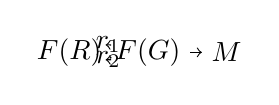
\begin{tikzpicture}
   \node (F1)               {$F(R)$};
   \node (F3) [right of=F1] {$F(G)$};
   \node (Q)  [right of=F3] {$M$};
   
   \path[->]
     (F1.10)  edge node        {$r_1$} (F3.170)
     (F1.350) edge node [swap] {$r_2$} (F3.190)
     (F3)     edge (Q);
  \end{tikzpicture}
 \end{center}
 ここで,$F(R)$と$F(G)$は自由モノイドであり,従って,
 $M \cong F(G)/(r_1=r_2)$ととなる.
\end{prop}
\begin{proof}
 任意のモノイド$N$に対し,$N$の元の集合上の自由モノイドを$TN = M(|N|)$と
 書く(従って$T$が函手となることに注意しよう).恒等射
 $1_{|N|}:|N| \to |N|$によって引き起こされる準同型
 \begin{align*}
  \pi: TN  &\to N\\
  \pi(x_1, \ldots, x_n) &= x_1 \cdot \ldots \cdot x_n
 \end{align*}
 が存在する.(ここでは明確化のため$TN$の元を文字列$x_1 \ldots x_n$では
 なく,タプル$(x_1, \ldots, x_n)$の形で書いた.)$T$を$M$に二回適用して,
 次の図式に示す射$\pi$と$\varepsilon$を得る.

 \begin{equation}\label{T2M図式}
  \tikzpicture
   \node (T2M)              {$T^2 M$};
   \node (TM) [right of=F1] {$TM$};
   \node (M)  [right of=F3] {$M$};

   \path[->]
     (T2M.10)  edge node        {$\varepsilon$} (TM.170)
     (T2M.350) edge node [swap] {$\mu$}         (TM.190)
     (TM)      edge node [swap] {$\pi$}          (M);
  \endtikzpicture
 \end{equation}
 ここで$T^2 M = TTM$かつ$\mu = T\pi$である.はっきりといえば,$T^2 M$の
 元は$M$の元のタプルのタプル,つまり
 $((x_1, \ldots, x_n), \ldots, (z_1, \ldots,z_m))$
 であり,準同型$\varepsilon$と$\mu$は次の効果を持つ.
 \begin{align*}
  \varepsilon((x_1, \ldots, x_n), \ldots, (z_1, \ldots,z_m))
    &= (x_1, \ldots, x_n, \ldots, z_1, \ldots,z_m)\\
  \mu((x_1, \ldots, x_n), \ldots, (z_1, \ldots,z_m))
    &= (x_1 \cdot \ldots \cdot x_n, \ldots, z_1 \cdot \ldots \cdot z_m)
 \end{align*}
 手短かにいえば,$\varepsilon$は$TM$の積を,$\mu$は$M$の積を使っている.

 ここで,明らかに$\pi \circ \varepsilon = \pi \circ \mu$である.
 (\ref{T2M図式})がモノイドのコイコライザとなることを示そう.そのために,
 モノイド$N$と$h\varepsilon = h\mu$なる準同型$h: TM \to N$が与えられたと
 しよう.すると,任意のタプル$(x, \ldots, z)$に対し,
 \begin{align}
  h(x, \ldots, z) &= h\varepsilon((x,\ldots, z))\notag\\
   &= h\mu((x, \ldots, z))\label{epsilon-and-mu}\\
   &= h(x \cdot \ldots \cdot z)\notag
 \end{align}
 が成立する.今,$i: |M| \to |TM|$を生成元の埋め込みとして,次の図式に示
 すように$\bar h = h \circ i$と定義しよう.
 \begin{center}
  \begin{tikzpicture}
   \node (T2M)              {$T^2 M$};
   \node (TM) [right of=F1] {$TM$};
   \node (M)  [right of=F3] {$M$};
   \node (N)  [below of=M]  {$N$};

   \path[->]
     (T2M.4)   edge node        {$\varepsilon$} (TM.175)
     (T2M.350) edge node [swap] {$\mu$}         (TM.190)
     (TM.10)   edge node        {$\pi$}         (M.165)
     (TM)      edge node [swap] {$h$}           (N)
     (M)       edge node        {$h \circ i$}   (N);
   \path[->, dotted]
     (M.200)   edge node        {$i$}           (TM.345);
  \end{tikzpicture}
 \end{center}
 すると,
 \begin{alignat*}{2}
   \bar h\pi(x,\ldots, z) &= hi\pi(x, \ldots, z) \\
    &= h(x \cdot \ldots \cdot z)\\
    &= h(x, \ldots, z) &\qquad \eqref{epsilon-and-mu}より
 \end{alignat*}

 $\bar h$が準同型となることは簡単な演習問題として読者に残しておこう
\end{proof}
\section{演習問題}
\begin{enumerate}
 \item 任意の圏${\bf C}$で,
       \begin{center}
	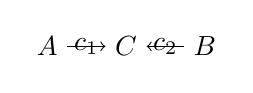
\begin{tikzpicture}
	 \node (A) {$A$};
	 \node(C) [right of=A]{$C$};\node(B) [right of=C]{$B$};
	 \path[->]
	   (A) edge node [swap] {$c_1$} (C)
           (B) edge node        {$c_2$} (C);
	\end{tikzpicture}
       \end{center}
       が余積図式となるのは,任意の対象$Z$に対して写像
       \begin{align*}
	\Hom(C, Z) &\to \Hom(A, Z) \times \Hom(B, Z)\\
	f &\mapsto \langle f \circ c_1, f \circ c_2 \rangle
       \end{align*}
       が同型となるとき,その時に限ることを示せ.直積での対応する事実と
       双対性を用いよ.
 \item 自由モノイド函手$M$が余積を保つことを詳しく示せ.つまり,任意の集
       合$A, B$について,
       \[
	M(A) + M(B) \cong M(A+B) \qquad (\text{標準的(canonically)})
       \]
       を示せ.教科書でほのめかした通り,余積$A+B$と$M(A)+M(B)$および自
       由モノイドの普遍写像性を使え.
 \item 教科書で説明した,モノイドの余積$A+B$を自由モノイド$M(|A|+|B|)$の
       商とする構成法が,実際にモノイドの圏での余積を与えていることを確
       かめよ.
 \item 二つの冪集合ブール代数$\Pow(A)$および$\Pow(B)$の直積が再び冪集合
       となること,すなわち集合$A$と$B$の余積の冪集合となることを示せ.
       \[
	\Pow(A) \times \Pow(B) \cong \Pow(A + B)
       \]
       (ヒント:射影$\pi_1: \Pow(A+B) \to \Pow(A)$および
       $\pi_2: \Pow(A+B) \to \Pow(B)$を決定し,これらが直積の普遍写像性
       を持つことを確かめよ.)
 \item 選言の導入規則と除去規則を持つ自然演繹系における証明からなる圏を
       考えよう.任意の$p: A \to C, q: B \to C $と $r: A+B \to C$に対し,
       等式
       \[
	[p, q] \circ i_1 = p,\qquad [p, q] \circ i_2 = q
       \]
       \[
        [r \circ i_1, r \circ i_2] = r
       \]
       によって証明を同一視する.これらの等式によって生成される(つまり一
       方の証明から上のような「脇道」をすべて取り除いて他方が得られたと
       き,二つの証明は等しくなるような)同値関係による証明の同値類を経
       由して得られる圏が,実際に余積を持つことを示せ.
 \item モノイドの圏は全てのイコライザと全ての有限直積を持つことを確かめ,
       アーベル群の圏についても同様のことを確かめよ.
 \item 余積を持つ任意の圏について,二つの射影的対象の余積は再び射影的と
       なることを確かめよ.
 \item 射影性の概念を双対化し,圏における{\bfseries 単射的}(injective)
       対象を定義せよ.posetの間の写像は元について単射であるとき,その時
       に限ってモノ射となることを示せ.単射的なposetとそうでないposetの
       例をそれぞれ与えよ.
 \item $\bar h$が実際に準同型となることを示して,教科書の命題
       \ref{Monoids are coeqs}の証明を完成させよ.
 \item 教科書の命題 \ref{Monoids are coeqs}の証明により,任意のモノイド
       は自由モノイドのコイコライザ$T^2M \rightrightarrows TM \to M$とし
       ての表示を持つことが示された.特にこの形のコイコライザは忘却函手
       $\Mon\to\Sets$によって保存されることを示せ.
 \item 次の方法でコイコライザを構成することで,$\Sets$は任意のコイコライ
       ザを持つことを示せ.任意の射の平行対のコイコライザ
       \begin{center}
	\begin{tikzpicture}
	 \matrix (m) [matrix of math nodes, column sep=1cm]{
	 A & B & Q=B/(f = g)\\
	 };
	 
	 \path[->]
	 (m-1-1.10)  edge node        {$f$} (m-1-2.170)
	 (m-1-1.350) edge node [swap] {$g$} (m-1-2.190)
	 (m-1-2)     edge (m-1-3);
	\end{tikzpicture}
       \end{center}
       を,任意の$x \in A$について$(f(x), g(x))$の対で生成される,
       $B$上の適切な同値関係$R$による$B$の商を取ることで構成せよ.(
       そうした対を全て含むようなすべての同値関係の共通部分として$R$を定
       義せよ.)
 \item 根つきposetの圏,即ち最小元$0$を持つposetと$0$を保つ単調写像の圏
       で余積を構成する際に言及した余積-コイコライザ構成を確かめよ.特に,
       そうした二つのposetの余積$P +_0 Q$は,posetの圏でのコイコライザ
       \begin{center}
	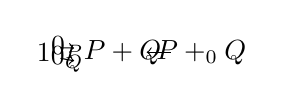
\begin{tikzpicture}
	 \node (1)   {$1$};
	 \node (P+Q)  [right of=1] {$P+Q$};
	 \node (P+0Q) [right of=P+Q] {$P +_0 Q$};
	 \path[->]
	   (1.15)  edge node {$0_P$} (P+Q.175)
	   (1.340) edge node [swap] {$0_Q$} (P+Q.190)
	   (P+Q)   edge (P+0Q);
	\end{tikzpicture}
       \end{center}
       として構成出来ることを示せ.(posetの圏は全てのコイコライザを持つ
       事実が与えられたとして示してもよい.)
 \item 次の手順に従って,モノイドの圏は全てのコイコライザを持つことを示
       せ.
       \begin{enumerate}
	\renewcommand{\labelenumii}{\arabic{enumii}. }
	\item 任意のモノイド準同型の組$f, g: M \to N$ が与えられたとき,
	      次の二つの$N$上の同値関係は一致することを示せ.
	      
	      \begin{enumerate}
	       \renewcommand{\labelenumiii}{(\alph{enumii}) }
	       \item $n \sim n' \Leftrightarrow$ 任意のモノイド$X$と準同
		     型$h: N \to X$について,$hf = hg$ならば$hn = hn'$が
		     成り立つ
	       \item 任意の$m \in M$ について $fm \sim gm$および
		     \[
		      n \sim n' \text{かつ} m \sim m' \Rightarrow
		       n \cdot m \sim n' \cdot m'
		     \]
		     が成立するような$N$上の同値関係$\sim$すべての共通部
		     分
	      \end{enumerate}
	\item $\sim$ を(1)で定義した同値関係とする.
	      このとき,$[n]\cdot[m] = [n \cdot m]$によって商集合
	      $N/\sim$はモノイドとなり,射影$N \to N/\sim$が$f$と$g$のコ
	      イコライザとなることを示せ.
       \end{enumerate}
 \item 集合の圏で次について考察せよ:
       \begin{enumerate}
	\item 写像$f: A \to B$が与えられたとき,写像$f \circ p_1, f
	      \circ p_2 : A \times A \to B$のイコライザを$A$上の(二項)
	      関係として説明し,同値関係となることを示せ(これは$f$の
	      {\bfseries 核}({\itshape kernel})と呼ばれる).
	\item 同値関係$R$による商写像$A \to A/R$の核は $R$ それ自身であ
	      ることを示せ.
	\item {\bfseries 任意の}二項関係$R \subseteq A \times A$に対し,
	      $\langle R \rangle$を$R$で生成される$A$上の同値関係
	      ($R$を含む最小の$A$上の同値関係)とする.このとき,商写像
	      $A \to A / \langle R \rangle$は二つの射影$R
	      \rightrightarrows A$のコイコライザとなることを示せ.
	\item 以上の議論を用いて,集合$A$上の任意の二項関係$R$に対し,
	      $R$で生成される同値関係$\langle R \rangle$は,$R$の二つの
	      射影のコイコライザの核として特徴付けられることを示せ.
       \end{enumerate}
 \item 次のようにして${\bf Top}$でコイコライザを構成せよ.二つの写像の平
       行対 $f, g: X \rightrightarrows Y$が与えられたとき,商空間
       $q: Y \to Q$を,(i)写像$|q|: |Y| \to |Q|$を得るために$\Sets$で
       $|f|$と$|g|$のコイコライザを取り,次に(ii)$|Q|$に商位相を入れる.
       つまり,$q^{-1}(V) \subseteq Y$が開集合のとき,その時にかぎって$V
       \subseteq Q$を開集合と定める.これは明らかに射影$|q|$を連続にする
       位相の中で最も精しい位相である.
\end{enumerate}
